\documentclass[tikz,border=8pt]{standalone}
% Shared look for every TikZ diagram. Load with % Shared look for every TikZ diagram. Load with % Shared look for every TikZ diagram. Load with \input{../../tools/tikz-style.tex}
\usepackage[T1]{fontenc}
\usepackage{lmodern}
\renewcommand{\sfdefault}{lmr}  % diagrams use the same serif as the text
\usetikzlibrary{arrows.meta, positioning, shapes.geometric, calc, fit, backgrounds}
\definecolor{cblue}{HTML}{4C78A8}
\definecolor{corange}{HTML}{F58518}
\definecolor{cgreen}{HTML}{54A24B}
\definecolor{cred}{HTML}{E45756}
\definecolor{cpurple}{HTML}{B279A2}
\definecolor{cgrey}{HTML}{6B6B6B}
\tikzset{
  every picture/.style={font=\sffamily, line width=1.2pt},
  box/.style={draw=#1, fill=#1!12, rounded corners=4pt, align=center, inner sep=7pt, minimum height=1.1cm},
  box/.default=cgrey,
  arrow/.style={-{Stealth[length=3mm]}, draw=cgrey, line width=1.4pt},
  title/.style={font=\sffamily\bfseries\Large},
  note/.style={font=\sffamily\small, text=cgrey, align=center},
}
\AtBeginDocument{\hyphenpenalty=10000 \exhyphenpenalty=10000}

\usepackage[T1]{fontenc}
\usepackage{lmodern}
\renewcommand{\sfdefault}{lmr}  % diagrams use the same serif as the text
\usetikzlibrary{arrows.meta, positioning, shapes.geometric, calc, fit, backgrounds}
\definecolor{cblue}{HTML}{4C78A8}
\definecolor{corange}{HTML}{F58518}
\definecolor{cgreen}{HTML}{54A24B}
\definecolor{cred}{HTML}{E45756}
\definecolor{cpurple}{HTML}{B279A2}
\definecolor{cgrey}{HTML}{6B6B6B}
\tikzset{
  every picture/.style={font=\sffamily, line width=1.2pt},
  box/.style={draw=#1, fill=#1!12, rounded corners=4pt, align=center, inner sep=7pt, minimum height=1.1cm},
  box/.default=cgrey,
  arrow/.style={-{Stealth[length=3mm]}, draw=cgrey, line width=1.4pt},
  title/.style={font=\sffamily\bfseries\Large},
  note/.style={font=\sffamily\small, text=cgrey, align=center},
}
\AtBeginDocument{\hyphenpenalty=10000 \exhyphenpenalty=10000}

\usepackage[T1]{fontenc}
\usepackage{lmodern}
\renewcommand{\sfdefault}{lmr}  % diagrams use the same serif as the text
\usetikzlibrary{arrows.meta, positioning, shapes.geometric, calc, fit, backgrounds}
\definecolor{cblue}{HTML}{4C78A8}
\definecolor{corange}{HTML}{F58518}
\definecolor{cgreen}{HTML}{54A24B}
\definecolor{cred}{HTML}{E45756}
\definecolor{cpurple}{HTML}{B279A2}
\definecolor{cgrey}{HTML}{6B6B6B}
\tikzset{
  every picture/.style={font=\sffamily, line width=1.2pt},
  box/.style={draw=#1, fill=#1!12, rounded corners=4pt, align=center, inner sep=7pt, minimum height=1.1cm},
  box/.default=cgrey,
  arrow/.style={-{Stealth[length=3mm]}, draw=cgrey, line width=1.4pt},
  title/.style={font=\sffamily\bfseries\Large},
  note/.style={font=\sffamily\small, text=cgrey, align=center},
}
\AtBeginDocument{\hyphenpenalty=10000 \exhyphenpenalty=10000}

\begin{document}
\begin{tikzpicture}[
  nd/.style={circle, draw=#1, fill=#1!15, minimum size=0.6cm, inner sep=0pt, line width=1pt},
  lab/.style={font=\sffamily\normalsize, align=center}]
  % column titles
  \node[title] at (3.0, 1.2) {Training};
  \node[title] at (11.0, 1.2) {Prediction};
  % row labels
  \node[lab, anchor=east, font=\sffamily\bfseries] at (-0.6, -0.6) {Original\\paper};
  \node[lab, anchor=east, font=\sffamily\bfseries] at (-0.6, -4.1) {Keras\\(inverted)};
  % ---- row 1: paper ----
  \node[nd=cblue] (a) at (0, -0.6) {}; \node[nd=cblue] (b) at (6, -0.6) {};
  \draw[arrow] (a) -- node[above, lab] {weight $w$} (b);
  \node[lab, text=cgrey] at (3, -1.6) {left node present in 75\% of steps, absent in 25\%};
  \node[nd=cblue] (c) at (8, -0.6) {}; \node[nd=cblue] (d) at (14, -0.6) {};
  \draw[arrow, draw=cgreen] (c) -- node[above, lab] {weight $w \times (1 - p) = 0.75\,w$} (d);
  \node[lab, text=cgrey] at (11, -1.6) {every node present: scale the weights down};
  % ---- row 2: Keras ----
  \node[nd=cblue] (e) at (0, -4.1) {}; \node[nd=cblue] (f) at (6, -4.1) {};
  \draw[arrow] (e) -- node[above, lab] {output $\times \dfrac{1}{1 - p} = \dfrac{1}{0.75}$} (f);
  \node[lab, text=cgrey] at (3, -5.1) {kept outputs scaled up while training};
  \node[nd=cblue] (g) at (8, -4.1) {}; \node[nd=cblue] (h) at (14, -4.1) {};
  \draw[arrow, draw=cgreen] (g) -- node[above, lab] {weight $w$, unchanged} (h);
  \node[lab, text=cgrey] at (11, -5.1) {every node present: nothing to do};
  \draw[cgrey!50, dashed, line width=0.8pt] (7.0, 1.6) -- (7.0, -5.6);
  \draw[cgrey!50, dashed, line width=0.8pt] (-2.4, -2.4) -- (14.4, -2.4);
  \node[note] at (6, -6.2) {dropout rate $p = 0.25$};
\end{tikzpicture}
\end{document}
